\chapter{Deformaci\'on de implantes de ortopedia} \label{ourapproach}

En el esquema CAOS propuesto en el cap\'itulo anterior, se mostraron siete etapas funcionales. Una de las etapas es llamada ``Deformaci\'on del implante'' la cual consiste en el moldeado del implante para que se adapte a una secci\'on del cuerpo. 

En este cap\'itulo, se estudiar\'a con m\'as detalle la deformaci\'on de las im\'agenes, trabajos previos en el \'area, la deformaci\'on de los implantes tratados como im\'agenes y el algoritmo empleado en nuestra propuesta. El estudio particular de esta etapa se debe a que mostramos un nuevo enfoque para la deformaci\'on de implantes que no estaba incluido en la t\'ecnica de MLS para deformaci\'on de im\'agenes. Nuestra propuesta realiza la deformaci\'on de los implantes de manera muy similar a como se realiza dentro de la sala de operaciones por el m\'edico cirujano.

%%%%%%%%%%%%%%%%%%%%%%%%%%%%%%%%%%%%%%%%%%%%%%%%
\section{Deformaci\'on de im\'agenes}

Definamos una imagen digital 2D, de dimensiones $M \times N$, como una funci\'on bidimensional $f$, donde $f(x,y)= C$ corresponde al valor del p\'ixel de la imagen en la posici\'on $(x,y)$, tal que $0 \le x \le M$ y $0 \le x \le N$.

Se puede definir el proceso de \textit{warping} de la imagen digital $U$ (origen) en la imagen $V$ (destino), como el proceso de la correspondencia de $f(U_x, Uy) = u(x,y)$ sobre el p\'ixel $f(V_x, Vy) = v(x,y)$, ver Figura \ref{fig:warping}.
\begin{figure}[htbp]
  \begin{center} \subfigure[]{\label{fig:warp1}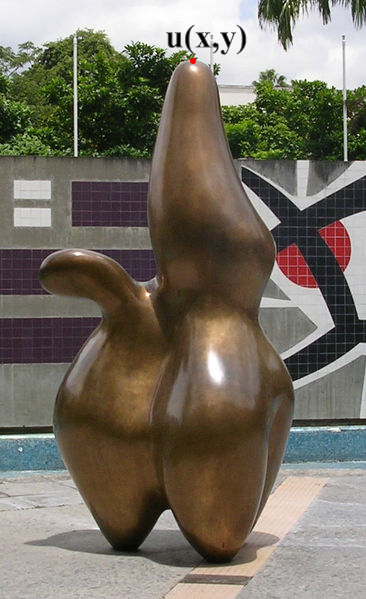
\includegraphics[width=0.30\columnwidth]{images/warp1.png}}  \subfigure[]{\label{fig:warp2}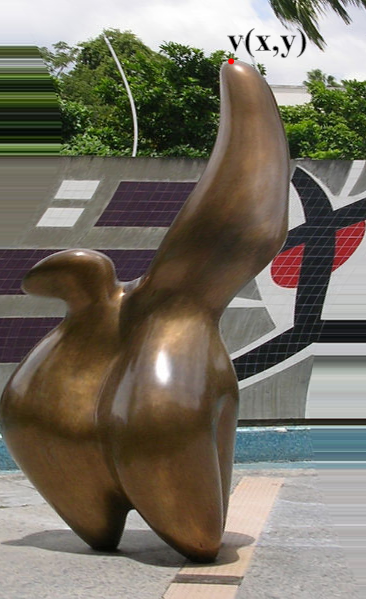
\includegraphics[width=0.30\columnwidth]{images/warp2.png}}   
  \end{center}
  \caption{\textit{Warping} de una imagen. (a) Imagen original (b) Imagen modificada}
  \label{fig:warping}
\end{figure}

Existen diversos enfoques para encontrar esta correspondencia entre $u(x,y)$ y $v(x,y)$, pero todos tienen como meta lograr una transici\'on suave con poca distorsi\'on visual. La deformaci\'on de im\'agenes (\textit{warping}) es una etapa importante en diversas aplicaciones en el procesamiento y an\'alisis de im\'agenes. Entre las aplicaciones que utilizan la deformaci\'on de im\'agenes se encuentran: el campo de la animaci\'on de personajes, el \textit{morphing} \cite{RUPE95}, im\'agenes m\'edicas \cite{KOBB03}, redimensionamiento de im\'agenes \cite{WANG08}, entre otros.

De acuerdo con Gomes et al. \cite{GOMES98}, los diferentes m\'etodos de \textit{warping} que han sido presentados en el \'area de Computaci\'on Gr\'afica pueden ser clasificados en 3 grupos:
\begin{enumerate}
	\item Basado en par\'ametros (\textit{parameter-based})
	\item Basado en forma libre (\textit{free-form based})
	\item Basado en rasgos (\textit{feature-based})
\end{enumerate}

Los m\'etodos basados en par\'ametros emplean transformaciones geom\'etricas globales. Una aplicaci\'on de ello se observa en operaciones como el doblado (\textit{bending}), torsi\'on (\textit{twisting}) y disminuci\'on de transformaciones.

Las t\'ecnicas basadas en forma libre utilizan curvas de forma libre para definir las transformaciones \textit{warping}. Uno de los primeros trabajos en esta \'area fue el realizado por Sederberg y Parry \cite{SEDE86}, donde se utiliz\'o una malla en conjunto con un pol\'igono controlador para realizar la deformaci\'on. Una subclase importante de este tipo de transformaciones, son las transformaciones de dos pasadas, las cuales reemplazan una transformaci\'on 2D por una secuencia de transformaciones ortogonales \textit{warping} m\'as simples.

Por \'ultimo, las t\'ecnicas basadas en rasgos emplean m\'etodos para localizar f\'acilmente bordes u otras discontinuidades, que son significativas para la geometr\'ia de los objetos a estudiar. Una colecci\'on de estas caracter\'isticas tanto en la imagen origen como en la destino, debe ser proporcionadas por el usuario. Un ejemplo de esta t\'ecnica es el algoritmo propuesto por Birkholz y Jack\`{e}l \cite{BIRK03} en donde se utilizan vectores como rasgos en la imagen, siendo su propuesta una mejora del trabajo de Beier y Neely \cite{BEIER92}. En la Figura \ref{fig:jackel} se muestra un ejemplo de la deformaci\'on hecha por Birkholz y Jack\`{e}l \cite{BIRK03}, donde se utiliza una curva como elemento modificador de la imagen.
\begin{figure}[htbp]
	\centering
	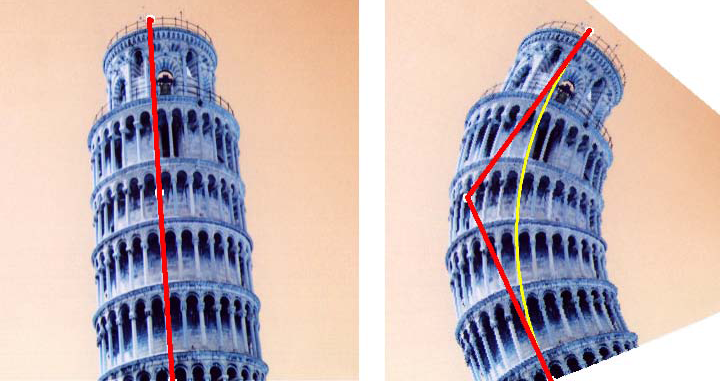
\includegraphics[width=.6\columnwidth]{images/jackel.png}
	\caption{Proceso de deformaci\'on controlado empleando una curva como rasgo caracter\'istico. Tomado de \cite{BIRK03}}
	\label{fig:jackel}
\end{figure}

Como se mencion\'o anteriormente, para realizar las t\'ecnicas basadas en rasgos, el usuario debe colocar un conjunto de identificadores para controlar dicha transformaci\'on. Estos identificadores pueden ser puntos, l\'ineas, curvas o un mallado. El usuario debe modificar la posici\'on y orientaci\'on de estos identificadores para conseguir que la imagen se deforme de una manera intuitiva.

En el presente cap\'itulo se estudiar\'a el proceso de \textit{warping}, as\'i como los trabajos realizados en el \'area, haciendo especial enfoque en la t\'ecnica empleada en este trabajo, denominada \textit{Moving Least Squares}. Al mismo tiempo, se mostrar\'a el trabajo realizado para la deformaci\'on de los implantes dentro de nuestro sistema CAOS.

%%%%%%%%%%%%%%%%%%%%%%%%%%%%%%%%%%%%%%%%%%%%%%
\section{Trabajos previos}

Los trabajos realizados en la deformaci\'on de im\'agenes tienen su principal inter\'es en la utilizaci\'on de diversos tipos de identificadores. Las t\'ecnicas basadas en mallas geom\'etricas como las deformaciones de forma libre \cite{SEDE86,LEES95}, parametrizan la imagen empleando splines bic\'ubicos bivariantes para crear deformaciones $C^2$. Usualmente este tipo de m\'etodos requieren alinear las l\'ineas de la malla que representan los puntos de control del spline con los identificadores seleccionados en una imagen, lo cual no resulta c\'omodo para el usuario.

En el a\~no 1992, Beier y Neely \cite{BEIER92} mejoraron el enfoque basado en mallas geom\'etricas y permitieron al usuario emplear un conjunto de l\'ineas. Dicho m\'etodo permite crear deformaciones suaves para conseguir un efecto final de \textit{morphing} o transici\'on entre 2 im\'agenes. En el trabajo de Beier y Neely se muestra adem\'as un efecto no deseado denominado \textit{fantasma} que consiste en pliegues no deseados en la deformaci\'on. Birkholz y Jack\`{e}l \cite{BIRK03} mejoraron la propuesta de Beier y Neely \cite{BEIER92} como se mencion\'o anteriormente.

Los algoritmos de deformaci\'on basados en rasgos asignan un valor de costo en cada identificador utilizado, pero no son ideales para realizar deformaciones basadas en el esqueleto de las figuras. Lewis et al. \cite{LEW00} presentaron un algoritmo para la deformaci\'on de formas basada en el esqueleto. El usuario controla la deformaci\'on del esqueleto y el resultado se alcanza de acuerdo con la correspondencia entre el esqueleto y la forma. El m\'etodo aplicado, obtiene mejores resultados en el movimiento de figuras de animales que de im\'agenes sin esqueleto. Sin embargo, la inicializaci\'on del esqueleto es una tarea compleja hecha por el usuario. En la Figura \ref{fig:lewis} se observa una deformaci\'on sobre un modelo que representa un brazo.
\begin{figure}[htbp]
  \begin{center} \subfigure[]{\label{fig:lewis1}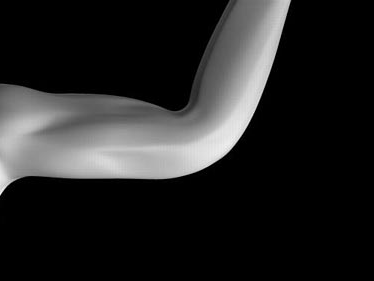
\includegraphics[width=0.30\columnwidth]{images/lewis1.png}}  \subfigure[]{\label{fig:lewis2}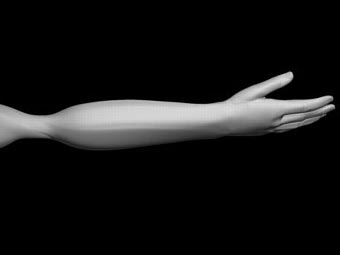
\includegraphics[width=0.30\columnwidth]{images/lewis2.png}}   
  \end{center}
  \caption{Deformaci\'on basada en esqueleto, propuesta por Lewis et al. \cite{LEW00} donde se muestra al modelo (a) doblando el codo y (b) girando el antebrazo}
  \label{fig:lewis}
\end{figure}

Weng et al. \cite{WENG06} presenta un algoritmo de deformaciones de formas 2D basado en la optimizaci�n de m\'inimos cuadrados no lineales, el cual alcanza resultados satisfactorios. A pesar de ello, este m\'etodo requiere un mayor costo computacional que el trabajo de Lewis et al. \cite{LEW00} y no contribuye considerablemente con el resultado de la deformaci\'on.

En el a\~no 2000, Alexa et al. \cite{ALEXA00} introducen el concepto de la transformaci\'on tan-r\'igida-como-sea-posible (\textit{as-rigid-as-possible}) que consiste en evitar las distorsiones indeseadas en una transformaci\'on tanto como sea posible, dejando que los escalamientos sean aplicados por transformaciones lineales. Para lograr esto, en el espacio de las deformaciones no se permiten escalas uniformes que distorsionen la imagen. 

Igarashi et al. \cite{IGAR05} propusieron una t\'ecnica interactiva que permite a un usuario realizar la deformaci\'on de una imagen 2D, empleando puntos como identificadores. En la Figura \ref{fig:iga} se observa una deformaci\'on de este tipo. Dicha t\'ecnica fue empleada para im\'agenes caricaturescas, cuyo resultado estuvo basado en el trabajo de Alexa et al. \cite{ALEXA00}, donde la deformaci\'on reduce al m\'inimo la cantidad de transformaciones de \textit{shear} y de escalado.
\begin{figure}[htbp]
  \begin{center} 
	  \subfigure[]{\label{fig:iga1}
\includegraphics[width=0.20\columnwidth]{images/iga1.png}}
	  \subfigure[]{\label{fig:iga2}
\includegraphics[width=0.20\columnwidth]{images/iga2.png}}
	  \subfigure[]{\label{fig:iga3}
\includegraphics[width=0.20\columnwidth]{images/iga3.png}}
  \end{center}
  \caption{Manipulaci\'on de una figura empleando puntos como identificadores. (a) Puntos blancos iniciales colocados dentro del objeto (b) y (c) Movimiento de los puntos por el usuario. Extra\'ido de \cite{IGAR05}}
  \label{fig:iga}
\end{figure}

En dicho trabajo, una malla triangular es empleada para representar la figura y el usuario debe mover los puntos identificadores. La posici\'on de los puntos identificadores que no son movidos en un momento dado, son calculados por minimizaci\'on de la distorsi\'on de cada tri\'angulo. Para resolver este problema como un problema lineal, se presenta un algoritmo de dos pasos: calcular la rotaci\'on y luego calcular el valor del escalado. Para producir la deformaci\'on \textit{as-rigid-as-possible}, Igarashi et al. \cite{IGAR05} realizan una triangulaci\'on de la imagen de entrada y resuelven un sistema de ecuaciones lineal cuyo tama\~no es igual al n\'umero de v\'ertices en la triangulaci\'on. 

En el a\~no 2006, Schaefer et al. \cite{SCHAF06} mejoran el trabajo de Igarashi et al. \cite{IGAR05} creando sistemas de ecuaciones de tama\~no $2x2$ en cada punto de inter\'es. Los puntos de inter\'es vienen dados por una malla uniforme rectil\'inea que cubre la imagen como se observa en la Figura \ref{fig:schafer}.
\begin{figure}[htbp]
  \begin{center} 
	  \subfigure[]{\label{fig:schafer1}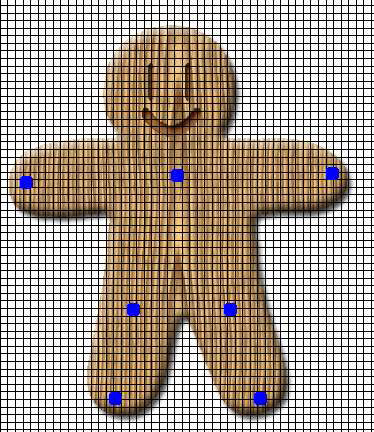
\includegraphics[width=0.30\columnwidth]{images/schafer1.png}}
	  \subfigure[]{\label{fig:schafer2}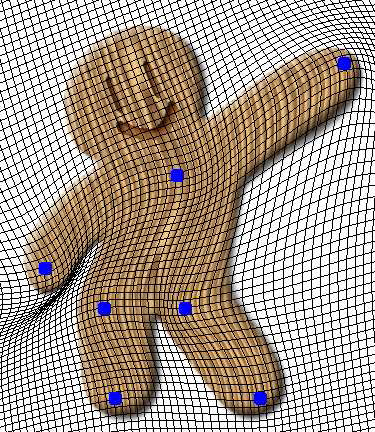
\includegraphics[width=0.30\columnwidth]{images/schafer2.png}}
  \end{center}
  \caption{Malla uniforme de $50 \times 50$ empleada por Schaefer et al. \cite{SCHAF06} para la deformaci\'on (a) Imagen original (b) Imagen al aplicar la deformaci\'on r\'igida.}
  \label{fig:schafer}
\end{figure}

En el trabajo propuesto por Schaefer et al. \cite{SCHAF06}, se plantean una serie de transformaciones distintas aplicadas a la deformaci\'on con m\'inimos cuadrados m\'oviles (\textit{Moving Least Square} - MLS). 

Nuestra propuesta est\'a basada en la t\'ecnica de MLS debido a que las t\'ecnicas mencionadas anteriormente trabajan sobre toda la imagen y no de forma local. Para la deformaci\'on dentro de nuestro sistema CAOS, se requiere de una deformaci\'on local en vez de una global. Por otra parte al utilizar una t\'ecnica basada en rasgos, es posible crear una interacci\'on con el usuario que permita realizar de manera sencilla una deformaci\'on dentro de nuestra propuesta. Al mismo tiempo, la t\'ecnica propuesta por Schaefer et al. \cite{SCHAF06} permite precalcular distintos valores previos a la ejecuci\'on del algoritmo en tiempo real. En la siguiente secci\'on, se describe la deformaci\'on empleada y cada una de las transformaciones que pueden ser aplicadas.

%%%%%%%%%%%%%%%%%%%%%%%%%%%%%%%%%%%%%%%%%%%%%%%%%%%%%%%%%%%%%%%%%
\section{Deformaci\'on con \textit{Moving Least Squares}}

El trabajo propuesto por Schaefer et al. \cite{SCHAF06} utiliza el concepto de \textit{Moving Least Squares} basado en la propuesta de Weng et al. \cite{WENG06} donde utilizan la optimizaci\'on no lineal de m\'inimos cuadrados. En dicho trabajo, el algoritmo propuesto se enfoca en preservar dos propiedades locales de la forma del objeto a deformar: las coordenadas laplacianas de los bordes y el \'area interior del objeto, ambas representadas por una funci\'on de energ\'ia no cuadr\'atica.

La deformaci\'on por m\'inimos cuadrados implementada por Weng et al. \cite{WENG06}, consiste en colocar una serie de puntos $p_i$ y $q_i$ y buscar la mejor transformaci\'on af\'in que logre minimizar el error en cuanto a las posiciones de estos puntos. En la Figura \ref{fig:cookie} se muestra un ejemplo de ello. La Figura \ref{fig:cookie1} es la imagen de entrada antes de la deformaci\'on, la Figura \ref{fig:cookie2} muestra el conjunto de puntos $p_i$ y $q_i$ ubicados en $R^2$ por $(x_i,y_i)$ y $(\hat{x_i},\hat{y_i})$ respectivamente, y la Figura \ref{fig:cookie3} muestra la deformaci\'on.

\begin{figure}[htbp]
  \begin{center}   \subfigure[]{\label{fig:cookie1}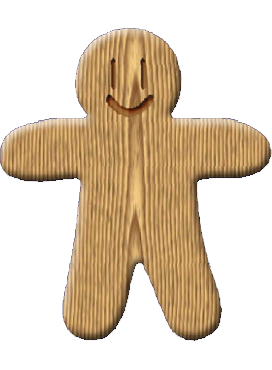
\includegraphics[width=0.25\columnwidth]{images/cookie.png}} \hspace{0.4cm} \subfigure[]{\label{fig:cookie2}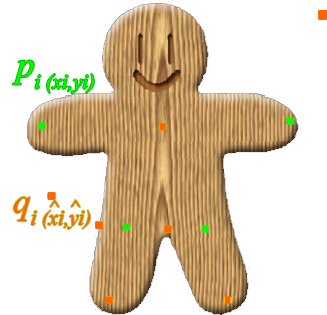
\includegraphics[width=0.30\columnwidth]{images/cookie2.png}} \hspace{0.4cm} \subfigure[]{\label{fig:cookie3}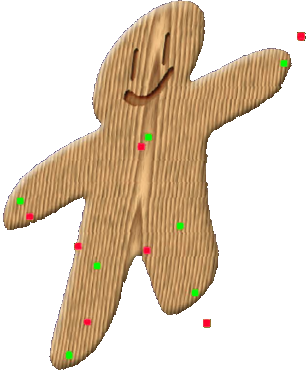
\includegraphics[width=0.255\columnwidth]{images/cookie3.png}}
  \end{center}
  \caption{Deformaci\'on empleando m\'inimos cuadrados. (a) Imagen original (b) Puntos $p_i$ y $q_i$ (c) Deformaci\'on aplicada}
  \label{fig:cookie}
\end{figure}

La deformaci\'on bajo \textit{Moving Least Squares} se puede definir como una funci\'on $f$ que satisface tres propiedades introducidas por Levin \cite{LEV98}:
\begin{itemize}
	\item Interpolaci\'on: Los puntos de control $p$ deben corresponder a los puntos $q$ luego de la deformaci\'on, i.e. $f(p_i)=q_i$.
	\item Suavidad: La funci\'on $f$ debe producir deformaciones con suavidad en la imagen.
	\item Identidad: Si el conjunto de puntos de control $p$ es el mismo conjunto $q$, entonces la funci\'on $f$ es la identidad.
\end{itemize}

Dichas propiedades permiten que los puntos de control sean interpolados y provean suavidad en el mismo. Al mismo tiempo, la propiedad de identidad garantiza el ajuste de la funci\'on $f$ con la mayor precisi\'on posible al momento de la aproximaci\'on de un punto deformado con respecto al original.

El objetivo de una transformaci\'on MLS es minimizar el error de la funci\'on de m\'inimos cuadrados que se obtiene en el proceso de correspondencia de los puntos $p_i$ con los puntos $q_i$. En este proceso, un conjunto de puntos de control son seleccionados dentro de la imagen origen y la funci\'on de transformaci\'on se obtiene para cada uno de estos puntos. Esta transformaci\'on est\'a basada en una funci\'on de pesos dentro de la funci\'on de m\'inimos cuadrados en cada punto de la evaluaci\'on.

Al utilizar las propiedades del \textit{Moving Least Squares} para la deformaci\'on de im\'agenes es posible encontrar, para un punto $v$ dentro de la imagen origen en $R^2$, la mejor transformaci\'on af\'in $l_v(x)$ que minimice la siguiente ecuaci\'on:
\begin{equation}
\label{ec:principal}
	\min_{l_v}\sum_i{w_i | l_v (p_i) - q_i |^2}
\end{equation}

En la Ec. \ref{ec:principal} $p_i$ y $q_i$ son vectores fila y los pesos $w_i$ son definidos de la siguiente forma:
\begin{equation}
\label{ec:ec1}
	w_i = \frac{1}{|p_i - v|^{2\alpha}}
\end{equation}

\noindent
donde $\alpha$ es una constante que permite aumentar o disminuir la tasa de decaimiento de la funci\'on de peso.

La funci\'on de deformaci\'on $f$ debe cumplir que $f(v) = l_v(x)$. Seg\'un Schaefer et al. \cite{SCHAF06}, la funci\'on $f$ cumple con las propiedades mencionadas anteriormente de la siguiente forma:
\begin{itemize}
	\item Interpolaci\'on: A medida que $v$ se aproxima a $p_i$ y $w_i$ se aproxima a infinito, la funci\'on $f$ es una funci\'on interpoladora, i.e., $f(p_i) = q_i$.
	\item Suavidad: La funci\'on de deformaci\'on $f$ tiene la propiedad de ser suave en cualquier punto a excepci\'on de los puntos de control $p_i$ donde $\alpha \le 1$.
	\item Identidad: Si $p_i = q_i$, entonces para todo $x$ se cumple que $l_v(x) = x$, obteniendo que $f(v) = v$.
\end{itemize}

Dado que $l_v(x)$ es una transformaci\'on af\'in entonces est\'a formada por una matriz de transformaci\'on lineal $M$ de $3 \times 3$ y un vector de traslaci\'on $T$ de $3 \times 1$ como se muestra en la Ecuaci\'on \ref{ec:afin}.
\begin{equation}
\label{ec:afin}
	l_v(x) = xM + T
\end{equation}

Es posible eliminar la traslaci\'on $T$ del problema de minimizaci\'on para simplificar las ecuaciones a resolver. Al sustituir la Ecuaci\'on \ref{ec:afin} en la Ecuaci\'on \ref{ec:principal}, \'esta se convierte en cuadr\'atica en $T$. Dado que el punto m\'inimo es donde las derivadas con respecto a cada una de las variables libres en $l_v(x)$ son iguales a cero, se puede resolver $T$ en t\'erminos de $M$. Si se toman las derivadas parciales con respecto a las variables libres en $T$ entonces se produce un sistema de ecuaciones lineales. Como se observa en la Ecuaci\'on \ref{ec:despe}, al despejar $T$ se obtiene:
\begin{equation}
\label{ec:despe}
	T = q_* - p_*M
\end{equation}

Los valores $p_*$ y $q_*$ son los puntos medios ponderados de todos los $p_i$ y $q_i$ calculados de la siguiente forma:
\begin{equation}
\begin{split}
	&p_* = \frac{\sum_i{w_ip_i}}{W}\\
  &q_* = \frac{\sum_i{w_iq_i}}{W}
\end{split}
\end{equation}

El valor de $W$ representa el peso total, y se calcula como $W = \sum{w_i}$. Si se sustituye el valor de $T$ dentro de la Ecuaci\'on \ref{ec:afin} y al escribir nuevamente la funci\'on $l_v$ en t\'erminos de la matriz lineal $M$ se obtiene:
\begin{equation}
\label{ec:linealm}
l_v(x) = (x - p_*)M + q_*
\end{equation}

Al utilizar el concepto anterior es posible reescribir el problema de los m\'inimos cuadrados en la Ecuaci\'on \ref{ec:principal} de la siguiente forma:
\begin{equation}
\label{ec:main}
\sum_i{w_i |\hat{p_i}M - \hat{q_i}|^2}
\end{equation}

En la Ecuaci\'on \ref{ec:main} los valores $\hat{p}$ y $\hat{q}$ se definen como $\hat{p} = p_i - p_*$ y $\hat{q} = q_i - q_*$. Dada la flexibilidad de la matriz $M$, es posible manejar transformaciones af\'ines, de similaridad o r\'igidas. En la Figura \ref{fig:deformation} se muestran los 3 tipos de transformaciones aplicadas a la deformaci\'on con MLS. A continuaci\'on se explican las transformaciones que pueden aplicarse en la matriz $M$.
\begin{figure}[htbp]
  \begin{center}   \subfigure[]{\label{fig:normalinput}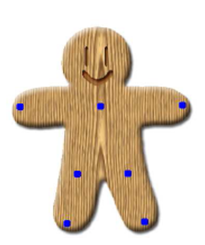
\includegraphics[width=0.23\columnwidth]{images/normalinput.png}}
\subfigure[]{\label{fig:affine}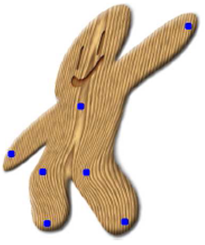
\includegraphics[width=0.23\columnwidth]{images/affine.png}} \hspace{0.2cm}
\subfigure[]{\label{fig:smilarity}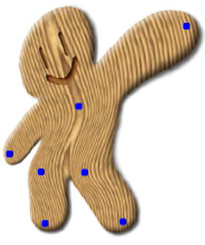
\includegraphics[width=0.23\columnwidth]{images/smilarity.png}}
\subfigure[]{\label{fig:rigid}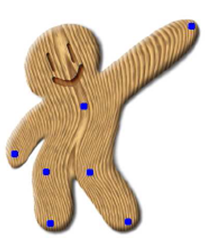
\includegraphics[width=0.23\columnwidth]{images/rigid.png}}
\end{center}
  \caption{Deformaci\'on empleando MLS. (a) Imagen original con los puntos de control en azul. (b) Deformaci\'on utilizando transformaci\'on af\'in, (c) transformaci\'on de similaridad y (d) transformaci\'on r\'igida}
  \label{fig:deformation}
\end{figure}

%%%%%%%%%%%%%%%%%%%%%%%%%%%%%%%%%%%%%%%%%%%
\subsection{Clases de transformaciones}

Las transformaciones aplicadas a la matriz $M$ se muestran como una soluci\'on a la funci\'on de deformaci\'on mostrada en la Ecuaci\'on \ref{ec:principal}. En las siguientes subsecciones, para cada transformaci\'on se muestra una forma cerrada de la soluci\'on que produce una r\'apida deformaci\'on de las im\'agenes.

%%%%%%%%%%%%%%%%%%%%%%%%%%%%%%%%%%%%%%%%%%%
\subsubsection{Transformaci\'on Af\'in}

Para emplear la transformaci\'on af\'in, la soluci\'on para la matriz $M$ se realiza empleando la ecuaci\'on normal:
\begin{equation}
\label{ec:tafin}
	M = \left(\sum_i{\hat{p}^T_i w_i \hat{p}_i}\right)^{-1} \sum_j{w_j\hat{p}^T_j \hat{q}_i}
\end{equation}

Para encontrar la soluci\'on a la Ecuaci\'on \ref{ec:tafin} se requiere la inversi\'on de una matriz, la cual es de tama\~no constante ($2 \times 2$ por trabajar con puntos 2D), haciendo este un proceso trivial. Con esta soluci\'on de forma cerrada para $M$, es posible escribir la funci\'on de deformaci\'on $f_a(v)$ como:
\begin{equation}
\label{ec:afinclosed}
	f_a(v) = (v - p_*)\left(\sum_i{\hat{p}^T_i w_i \hat{p}_i}\right)^{-1} \sum_j{w_j\hat{p}^T_j \hat{q}_i} + q_*
\end{equation}

Al aplicar esta funci\'on de deformaci\'on en cada punto de la imagen, se crea una nueva imagen deformada. Dicha imagen, se crea por la interacci\'on del usuario al manipular los puntos $ q_i$ de la imagen origen; los puntos $p_i$ se mantienen fijos. Dado que los puntos $p_i$ no son modificados, es posible calcular previamentelos valores que se muestran en la Ecuaci\'on \ref{ec:afinclosed} para obtener las deformaciones de forma m\'as r\'apida.

Simplificando la Ecuaci\'on \ref{ec:afinclosed} tenemos que:
\begin{equation}
\label{ec:ec3}
\begin{split}
	f_a(v) &= \sum_i{A_j \hat{q}_j + q_{*}} \\
  A_{j} &= (v - p_{*})\left( \sum_i{\hat{p}_i^T w_i \hat{p}_i} \right)^{-1} \hat{p}_j^T 
\end{split}
\end{equation}

La deformaci\'on af\'in est\'a formada por escalamientos no uniformes y transformaciones \textit{shear}, creando resultados visuales no deseados (artefactos). Para solucionar este problema, es necesario considerar ciertas restricciones a la transformaci\'on lineal $l_v(x)$, las cuales llevan a la transformaci\'on de similaridad y a la transformaci\'on de cuerpos r\'igidos.

%%%%%%%%%%%%%%%%%%%%%%%%%%%%%%%%%%%%%%%%%%%
\subsubsection{Transformaci\'on de Similaridad}

Las transformaciones de similaridad son un subconjunto de las transformaciones af\'ines que incluyen traslaci\'on, rotaci\'on y escalamiento uniforme, pero eliminando la transformaci\'on \textit{shear} de la deformaci\'on.

La restricci\'on aplicada en la deformaci\'on de similaridad es sobre la matriz $M$. La matriz debe tener la propiedad de que $M^T M = \lambda^2 I$ para alg\'un escalar $\lambda$. Si la matriz $M$ puede ser definida como una matriz en bloque de la forma:
$$M = \left(M_1\mbox{   }M_2\right)$$

\noindent
donde $M_1$, $M_2$ son vectores columnas de longitud 2, entonces se aplica la restricci\'on $M_1^T M_2 = 0$ tal que $M_2=M1^{\perp}$ donde el operador $\perp$ viene definido por la operaci\'on $(x,y)^{\perp} = (-y,x)$.

Dado que el problema de m\'inimos cuadrados a resolver, se mantiene cuadr\'atico en $M_1$, entonces el objetivo es minimizar la siguiente ecuaci\'on:
\begin{equation}
\label{ec:lepsimilarity}
\sum_i{wi \mid \left( \begin{array}{cc} \hat{p}_i \\ -\hat{p}_i^{\perp} \end{array} \right) M_1 - \hat{q}_i^T \mid^2}
\end{equation}

La funci\'on de la Ecuaci\'on \ref{ec:lepsimilarity} tiene un \'unico valor m\'inimo, el cual crea una transformaci\'on \'optima para la matriz $M$:
\begin{equation}
\label{ec:Msimilarity}
M = \frac{1}{\mu_s} \sum_i{w_i \left( \begin{array}{cc} \hat{p}_i \\ -\hat{p}_i^{\perp} \end{array} \right) (\hat{q}_i^T \mbox{    } -\hat{q}_i^{\perp T})}
\end{equation}
donde
$$ \mu_s = \sum_i{w_i \hat{p}_i \hat{p}_i^T} $$
Entonces, la soluci\'on para la funci\'on de deformaci\'on de similaridad $f_s$ puede ser calculada como:
\begin{equation}
\label{ec:fs}
	f_s(v) = \sum_i{\hat{q}_i \left( \frac{1}{\mu_s}A_i \right) + q_*}
\end{equation}
\begin{equation}
\label{ec:matrixA}
	A_i = w_i \left( \begin{array}{cc} \hat{p}_i \\ \hat{p}_i^{\perp} \end{array} \right)\left( 		\begin{array}{cc} v - p_* \\ -(v - p_*)^{\perp} \end{array} \right)^T
\end{equation}

La forma de la Ecuaci\'on \ref{ec:fs} permite precalcular la mayor cantidad de informaci\'on tal como se hace en la transformaci\'on af\'in. La deformaci\'on de similaridad preserva los \'angulos de la imagen original mejor que la deformaci\'on af\'in. Sin embargo, permitir el escalado de valores locales puede causar deformaciones indeseables a nivel visual en algunas oportunidades. Para eliminar estos posibles artefactos, las deformaciones r\'igidas son presentadas como una soluci\'on.

%%%%%%%%%%%%%%%%%%%%%%%%%%%%%%%%%%%%%%%%%%%
\subsubsection{Transformaci\'on R\'igida}

La matriz de transformaci\'on para la deformaci\'on \textit{as-rigid-as-possible} se obtiene al eliminar la restricci\'on del escalamiento uniforme. La soluci\'on propuesta por Schaefer et al. \cite{SCHAF06} muestra una soluci\'on simple y en su forma cerrada. Esta transformaci\'on puede ser obtenida con una peque\~na modificaci\'on de la transformaci\'on de similaridad, y es que la modificaci\'on consiste en aplicar una restricci\'on a la matriz $M$, la cual debe satisfacer que $M^T M = lambda^2I$ para alg\'un escalar $\lambda$.

Ahora, si la matriz $M$ puede ser definida como una matriz de bloque de la forma:
\begin{equation} 
M = (M_1 \mbox{  }M_2) 
 \end{equation}
 
\noindent
donde $M_1$ y $M_2$ son vectores columna de tama\~no 2, entonces la restricci\'on sobre $M$ requiere que se cumpla que $M_1^T M_2 = 0$, lo cual implica que $M_2 = M_1^{\bot}$.

Para satisfacer la condici\'on de rigidez $M^T M = \lambda^2I$, las constantes de escalamientos deben ser eliminadas. Al utilizar derivadas parciales con respecto a las variables libres de $M$ y sustituyendo los valores dentro de la funci\'on de error, la transformaci\'on es la mostrada en la Ecuaci\'on \ref{ec:Msimilarity} a excepci\'on de la constante $\mu_s$, que cambiaremos por $\mu_r$, como sigue:
\begin{equation} 
 \mu_r = \sqrt{\left( \sum_i{w_i \hat{q}_i \hat{p}_i^T} \right)^2 + \left( \sum_i{w_i \hat{q}_i \hat{p}_i^{\perp T}} \right)^2} 
 \end{equation}

En la transformaci\'on r\'igida, se define un vector de deformaci\'on r\'igida $\vec{f_r(v)}$, el cual es una versi\'on rotada y escalada del vector $v - p_*$ definido como:
\begin{equation} 
\label{ec:rigidandA}
	\vec{f_r(v)} =  \sum_i{\hat{q}_i A_i}
\end{equation}

La matriz $A$ es la misma utilizada en la Ecuaci\'on \ref{ec:matrixA}. Entonces, para calcular la funci\'on $f_r(v)$ se procede de la siguiente forma:
\begin{equation} 
\label{ec:rigidtransf}
	f_r(v) = \mid v - p_*\mid \frac{\vec{f_r(v)}}{\mid \vec{f_r(v)} \mid} + q_*
\end{equation}

Esta transformaci\'on es computacionalmente m\'as lenta en comparaci\'on con la transformaci\'on de similaridad al incluir el factor de la normalizaci\'on por $\vec{f_r(v)}$. En la Figura \ref{fig:pisa} se puede observar la deformaci\'on de una imagen 2D aplicando cada una de las transformaciones explicadas. Cabe destacar, que la transformaci\'on de rigidez preserva los \'angulos y la forma del objeto mejor que la transformaci\'on af\'in y de similaridad, desde el punto de vista visual.

\begin{figure}[htbp]
  \begin{center}   \subfigure[]{\label{fig:pisa0}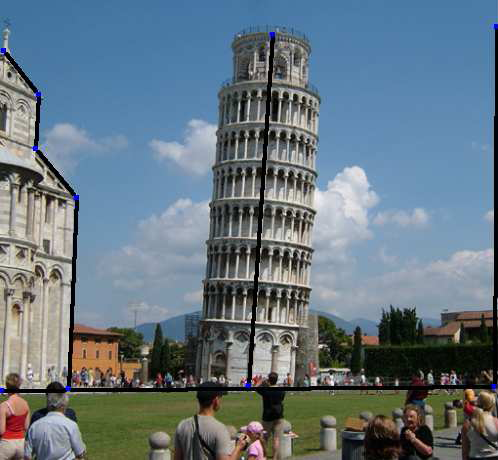
\includegraphics[width=0.24\columnwidth]{images/pisa0.png}}
\subfigure[]{\label{fig:pisa1}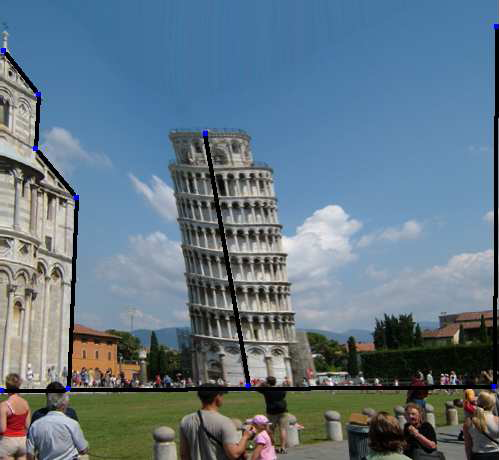
\includegraphics[width=0.24\columnwidth]{images/pisa1.png}}
\subfigure[]{\label{fig:pisa2}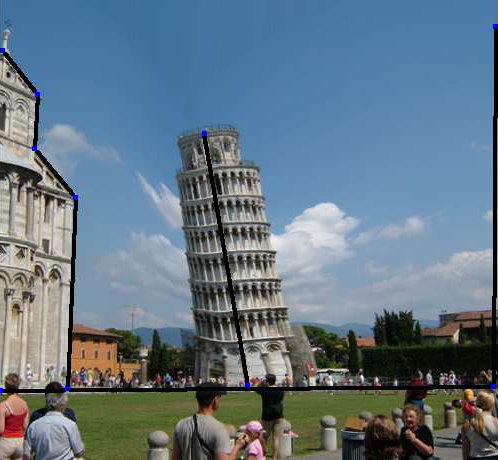
\includegraphics[width=0.24\columnwidth]{images/pisa2.png}}
\subfigure[]{\label{fig:pisa3}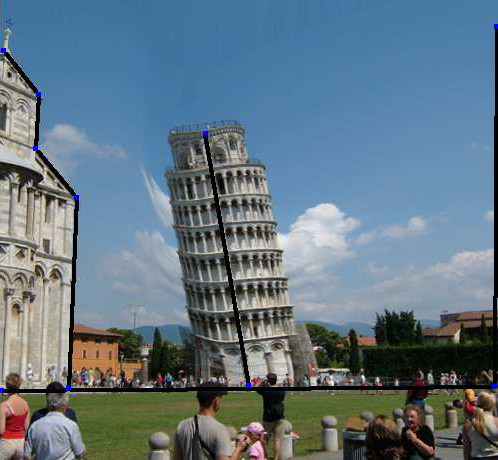
\includegraphics[width=0.24\columnwidth]{images/pisa3.png}}
\end{center}
  \caption{Deformaci\'on de la Torre de Pisa empleando MLS (extra\'ido de \cite{SCHAF06}). (a) Imagen original. (b) Deformaci\'on con transformaci\'on Af\'in (c) Deformaci\'on con transformaci\'on de Similaridad (d) Deformaci\'on con transformaci\'on R\'igida}
  \label{fig:pisa}
\end{figure}

\section{Deformaci\'on de los implantes}

%%%%%%%%%%%%%%%%%%%%%%%%%%%%%%%%%%%%%%%%%%%%
\subsection{Trabajos previos}

Michal\'{i}kov\'{a} et al. \cite{MILA10} define la planificaci\'on preoperatoria digital como un proceso r\'apido, preciso y eficiente. El objetivo principal de dicho procedimiento es mejorar el resultado de la operaci\'on en una sala de cirug\'ia y su efecto sobre el paciente. Adem\'as, \'esta provee un historial cl\'inico del procedimiento quir\'urgico.

Algunas \'areas de la medicina actual, emplean la planificaci\'on preoperatoria como parte esencial de su pr\'actica diaria. Un caso notable de este tipo de sistemas CAOS es el mostrado para la planificaci\'on preoperatoria para el reemplazo total de rodilla presentado por Friederich y Verdonk \cite{FRIED08}. En dicho trabajo, \'estos determinan la importancia de un sistema CAOS como una herramienta para conseguir un alineamiento correcto de una pr\'otesis a ser colocada en el paciente.

Oll\'e et al. \cite{OLLE06} desarrollan un sistema para la planificaci\'on preoperatoria basado en im\'agenes de huesos fracturados. Su propuesta se basa en un esquema donde im\'agenes de CT son utilizadas como entrada al sistema. Luego, dichas im\'agenes son segmentadas para realizar una extracci\'on de una isosuperficie. Una vez obtenida la isosuperficie, los cirujanos pueden colocar implantes mientras realizan una operaci\'on virtual sobre los huesos fracturados. En la Figura \ref{fig:olle} se muestra la colocaci\'on de implantes en el modelo de huesos de una mu\~neca, producida por Oll\'e et al. \cite{OLLE06}. En dicho trabajo, se realiza un c\'alculo de an\'alisis de esfuerzo utilizando Elementos Finitos con el objetivo de verificar que la estrategia quir\'urgica sea efectiva.
\begin{figure}[htbp]
  \begin{center}
  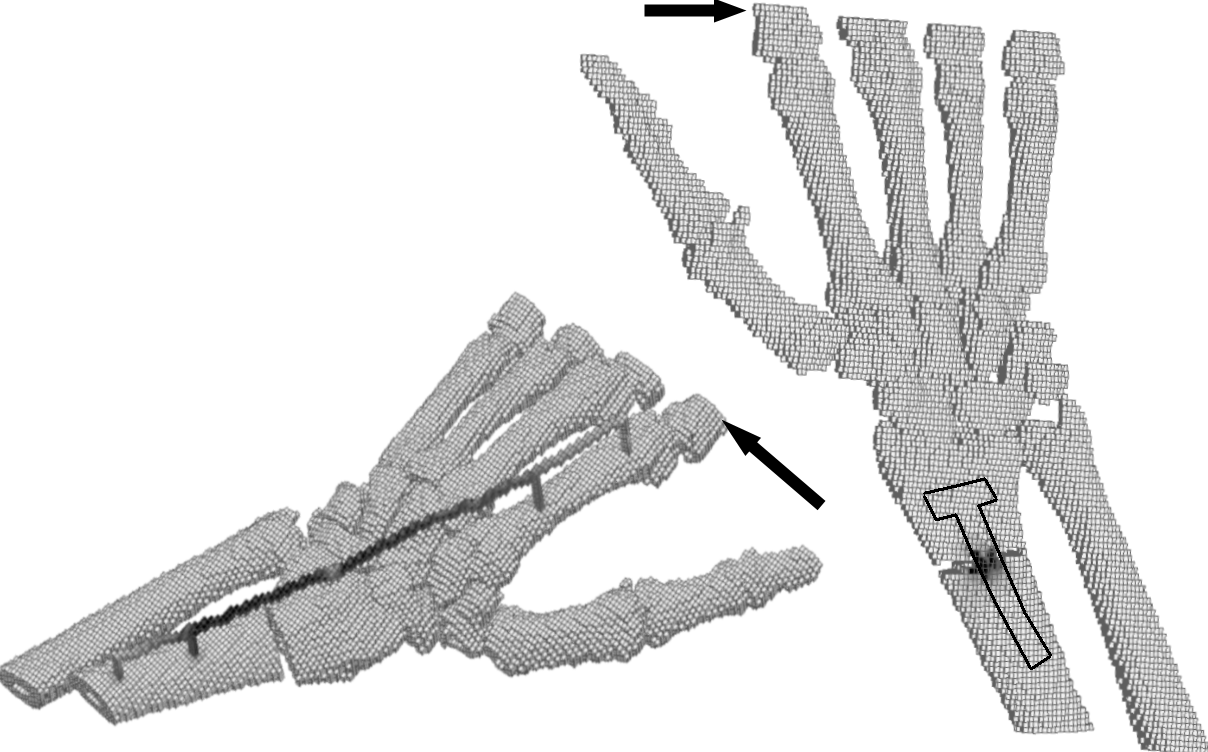
\includegraphics[width=.6\columnwidth]{images/olle.png}
  \caption{Mu\~neca con una fractura artificial despu\'es de la aplicaci\'on de una fijaci\'on externa (izquierda) y de una placa en forma de T (derecha). Imagen tomada de \cite{OLLE06}}
  \label{fig:olle}
  \end{center}
\end{figure}

Estos dos trabajos mencionados anteriormente, utilizan datos 3D de los pacientes provenientes de una CT como entrada. Dichos datos son adquiridos desde diversos equipos de adquisici\'on. Sin embargo, no todos los sistemas de planificaci\'on preoperatoria trabajan solo con im\'agenes 3D. Existe otra categor\'ia de estos sistemas que se basa en im\'agenes 2D tomadas de los pacientes, como las radiograf\'ias convencionales.

Un ejemplo de este tipo de investigaci\'on es la presentada por Steinberg et al. \cite{STEI10} el cual describe como satisfactorio los resultados obtenidos en la planificaci\'on preoperatoria de reemplazo de cadera. En dicho trabajo se utiliz\'o im\'agenes 2D de Rayos-X. Otro trabajo destacado, es el presentado por Jamali \cite{JAMA09} quien presenta una planificaci\'on preoperatoria de cirug\'ia empleando radiograf\'ias est\'andares y plantillas 2D de implantes.

En algunos casos, es necesario deformar los implantes para obtener una mejor planificaci\'on que simule la cirug\'ia de manera fidedigna. Korner et al. \cite{KORN03} afirman que en la mayor\'ia de los casos donde las fracturas est\'an ubicadas cerca de las articulaciones y el paciente requiere de un proceso de fijaci\'on con placas, dicha placa necesita ser doblada. 

En la pr\'actica los cirujanos deben invertir una cantidad de tiempo en realizar este proceso y en muchas ocasiones, repetir muchas veces el procedimiento (doblado-colocaci\'on) hasta obtener la mejor fijaci\'on para el implante. Un trabajo relevante en esta \'area fue presentado por Sagbo et al. \cite{SAGBO051}, quienes implementan diversos algoritmos cl\'asicos para el doblado de implantes representados como una geometr\'ia 3D (ver Figura \ref{fig:sagbo1}). Los algoritmos implementados son clasificados en dos grupos: m\'etodos geom\'etricos y m\'etodos f\'isicos. El objetivo final de estos algoritmos es ser integrados en un planificador de operaciones ortop\'edico creado por dichos autores. El proceso de deformaci\'on mostrado por Sagbo et al. \cite{SAGBO051} est\'a pensado para im\'agenes 3D, donde se puede realizar operaciones de rotaci\'on en 3D sobre la fractura y los implantes (i.e. isosuperficies y vol\'umenes).
 \begin{figure}[htbp]
  \begin{center}
  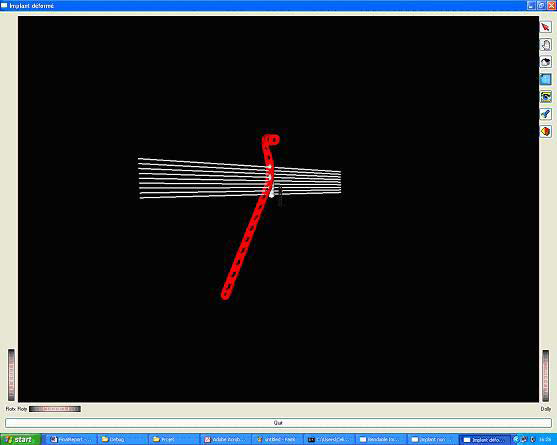
\includegraphics[width=.6\columnwidth]{images/sagbo1.png}
  \caption{Doblado de un implante donde se muestran diez puntos de control para la deformaci\'on). Tomada de \cite{SAGBO051}}
  \label{fig:sagbo1}
  \end{center}
\end{figure}

Sin embargo, muchos algoritmos para la deformaci\'on de im\'agenes en 2D han sido desarrollados. Una importante contribuci\'on en esta \'area fue introducida por Schaefer et al. \cite{SCHAF06}, los cuales proponen una deformaci\'on de im\'agenes basada en MLS. Dicho trabajo, es una mejora del trabajo propuesto por Igarashi et al. \cite{IGAR05}.

En \cite{RAM10} se present\'o un esquema de planificaci\'on preoperatoria que considera la deformaci\'on de las im\'agenes, empleando im\'agenes 2D como entrada. En dicho trabajo, se utiliza la t\'ecnica de deformaci\'on basada en el trabajo de Birkholz y Jack\`{e}l \cite{BIRK03}, pero esta no produce un resultado visual aceptable ya que deforma la imagen completa. En la pr\'actica al realizar el doblado de los implantes, los cirujanos requieren una deformaci\'on local solo en el \'area de inter\'es. En este trabajo se presenta un nuevo m\'etodo para la deformaci\'on de implantes en nuestra propuesta de sistema CAOS la cual est\'a enfocada en fracturas de los miembros inferiores. Este m\'etodo es una nueva variante de la t\'ecnica de MLS para la deformaci\'on de im\'agenes 2D. A continuaci\'on se explica con detalle el esquema propuesto para la deformaci\'on de los implantes de ortopedia.

%%%%%%%%%%%%%%%%%%%%%%%%%%%%%%%%%%%%%%%%%%%%
\subsection{Esquema propuesto}

En la Figura \ref{fig:pipeline} se muestra el flujo de trabajo empleado para la deformaci\'on de los implantes en nuestra propuesta de sistema CAOS. A continuaci\'on	se describe cada una de las etapas de este flujo de trabajo.

\begin{figure}[htb]
	\centering
	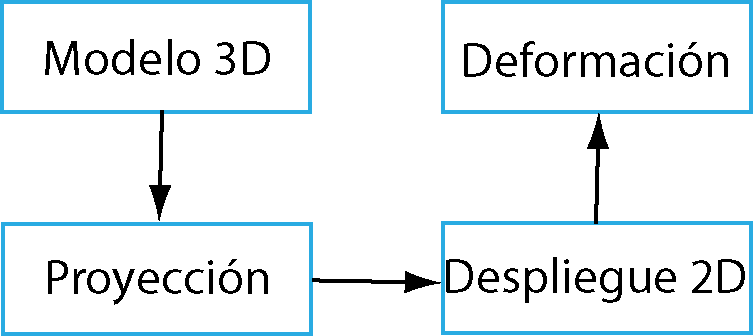
\includegraphics[width=0.5\columnwidth]{images/pipeline.png}
	\caption{Flujo de trabajo empleado para la deformaci\'on de los implantes}
	\label{fig:pipeline}
\end{figure}

%%%%%%%%%%%%%%%%%%%%%%%%%%%%%
\subsubsection{Modelo 3D}
El implante utilizado en nuestra propuesta de sistema CAOS, es generado empleando el software Autodesk Inventor \textsuperscript{\texttrademark} \cite{website:inventor}. Dicho software es una herramienta de construcci\'on de modelos geom\'etricos especializada para cualquier tipo de piezas. Particularmente, las piezas empleadas en este trabajo son como la mostrada en la Figura \ref{fig:inventor}.

\begin{figure}[htb]
	\centering
	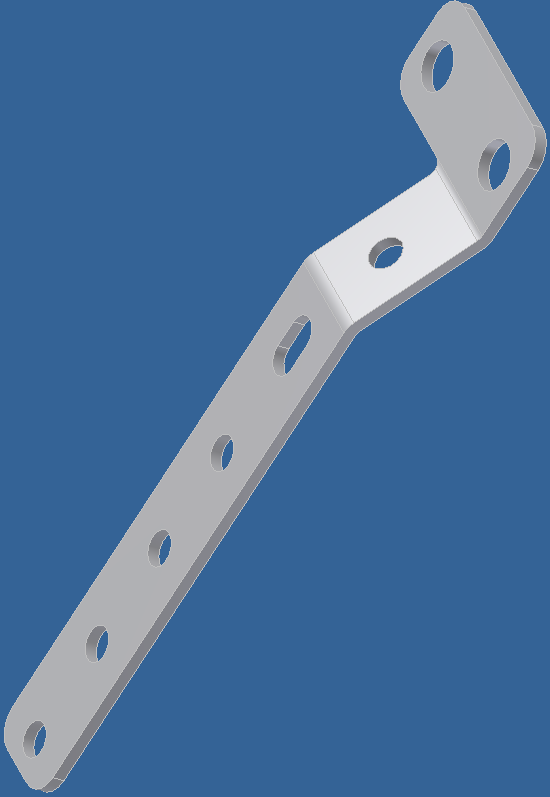
\includegraphics[width=0.3\columnwidth]{images/inventor.png}
	\caption{Implante de una pieza de osteos\'intesis creada en Autodesk Inventor \textsuperscript{\texttrademark} \cite{website:inventor}}
	\label{fig:inventor}
\end{figure}

Cada pieza est\'a representada por una geometr\'ia basada en un mallado de pol\'igonos. El formato de archivo utilizado fue STL (\textit{stereolithography}), el cual consta de una representaci\'on sencilla para el manejo de geometr\'ias. Es posible generar el archivo en formato STL en tres distintas resoluciones: baja, media y alta. El objetivo de esto es obtener mayor refinamiento al momento de modelar la pieza. A mayor resoluci\'on, mayor es la cantidad de pol\'igonos que forman dicha estructura.

Posteriormente, se obtiene un implante que el usuario selecciona y este act\'ua como entrada a la etapa de \textit{Proyecci\'on}.

%%%%%%%%%%%%%%%%%%%%%%%%%%%%%
\subsubsection{Proyecci\'on}
Una vez que el usuario ha cargado el implante dentro del sistema CAOS, se selecciona cu\'al de las diferentes vistas desea utilizar. Dichas vistas corresponden a una proyecci\'on ortogonal sobre cada una de las caras de la caja envolvente donde yace el implante.

La proyecci\'on ortogonal se realiza sobre los planos $xy$, $yz$ y $xz$ en coordenadas de ojo dentro del proceso de visualizaci\'on. La caja que envuelve al implante (en coordenadas 3D) corresponde a un paralelep\'ipedo, el cual tiene diferentes dimensiones de ancho $w$, alto $h$ y profundidad $d$. Al realizar la proyecci\'on sobre el plano de proyecci\'on se modifican las dimensiones de dicho plano con el objetivo de ajustarlo al tama\~no del mismo. Por ejemplo, si la caja envolvente tiene las dimensiones $w=20$, $h=20$ y $d=10$ y es proyectado sobre el plano $xz$ las dimensiones del plano de proyecci\'on ser\'an $w=1$, $h=0.5$ y $d=0$.

Luego de ser proyectado sobre el plano, se procede a aplicar las transformaciones correspondientes para llevar el objeto proyectado al dispositivo de salida (en coordenadas 2D).

%%%%%%%%%%%%%%%%%%%%%%%%%%%%%
\subsubsection{Despliegue 2D}
Con la proyecci\'on obtenida se realiza una correspondencia entre el plano de proyecci\'on y una imagen en formato RGBA. El canal de transparencia permite superponer el implante sobre la planificaci\'on preoperatoria. El resultado de la proyecci\'on es ubicado en una imagen de dimensiones $w \times h$, que corresponde a las medidas dentro de la planificaci\'on de acuerdo a la calibraci\'on realizada. En la Figura \ref{fig:placeimplant} se observa el implante colocado sobre la imagen de la planificaci\'on.

\begin{figure}[htb]
	\centering
	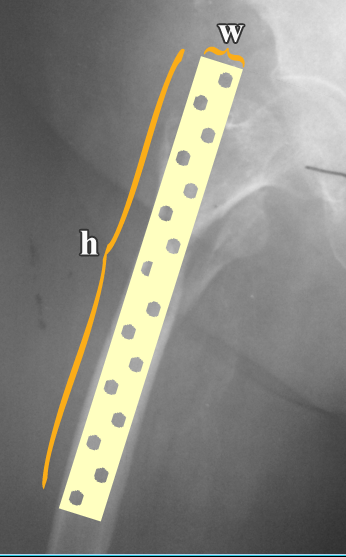
\includegraphics[width=0.20\columnwidth]{images/placeimplant.png}
	\caption{Ubicaci\'on de una imagen del implante sobre una planificaci\'on preoperatoria}
	\label{fig:placeimplant}
\end{figure}

Las dimensiones que debe tener un implante, es decir, los valores $(w,h,d)$ se encuentran almacenados en la descripci\'on del implante dentro de una base de datos MySQL. Para cada implante se almacena su ubicaci\'on dentro del sistema de archivos y sus medidas. El proceso de agregar un nuevo implante, se realiza a trav\'es del software de nuestro sistema CAOS donde se debe indicar cada una de las medidas para el ancho, largo y profundidad de un implante.

Cuando el implante se encuentra sobre la imagen en la cual se est\'a trabajando, la deformaci\'on se realiza en un espacio de imagen 2D. A continuaci\'on se describe como se realiza dicho proceso de deformaci\'on.

%%%%%%%%%%%%%%%%%%%%%%%%%%%%%
\subsubsection{Deformaci\'on}

Con la imagen del implante sobre la planificaci\'on, se coloca una serie de \textit{controladores} para que el usuario pueda modificarlos y realizar la deformaci\'on. Estos controladores son definidos por puntos sobre una curva localizada en el eje mayor de mayor longitud del implante. En la Figura \ref{fig:handler} se observa un ejemplo de la ubicaci\'on de los controladores.
\begin{figure}[htbp]
  \begin{center} 
  	\subfigure[]{\label{fig:handler1}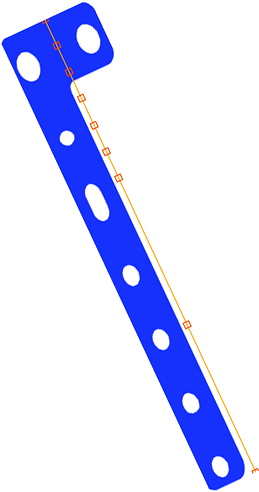
\includegraphics[width=0.20\columnwidth]{images/handlers3.png}} \hspace{1.6cm}
  	\subfigure[]{\label{fig:handler2}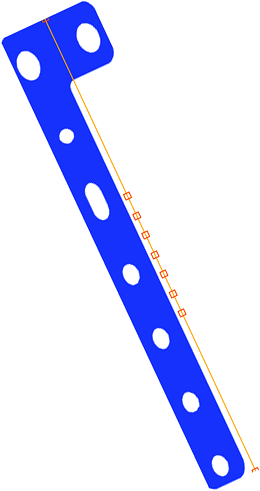
\includegraphics[width=0.20\columnwidth]{images/handlers2.png}} \hspace{1.6cm}
  	\subfigure[]{\label{fig:handler3}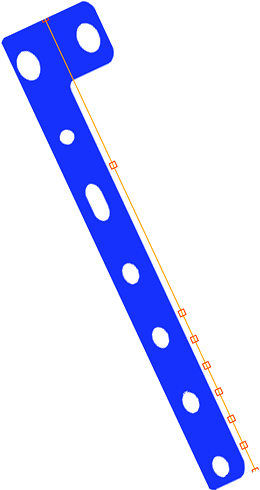
\includegraphics[width=0.20\columnwidth]{images/handlers1.png}}
  \end{center}
  \caption{Controladores sobre la imagen del implante. La ubicaci\'on de la mayor\'ia de los controladores de acuerdo a donde se va a realizar la deformaci\'on: (a) izquierda, (b) centro, (c) derecha}
  \label{fig:handler}
\end{figure}

Es posible realizar una distribuci\'on uniforme de los controladores sobre el eje central o una mayor distribuci\'on sobre los extremos para tener m\'as precisi\'on en los extremos del implante y as\'i tener un control local de la deformaci\'on.

Los controladores pueden ser modificados con el objetivo de modificar la imagen. El movimiento de los controladores es realizado por el m\'edico usuario del sistema CAOS, pudiendo ser desplazados solamente en dos sentidos: hacia arriba y hacia abajo.

En la Figura \ref{fig:points1} se observa un ejemplo de tres controladores sobre una curva. Los movimientos para la deformaci\'on se realizan solo hacia arriba o hacia abajo, ver Figura \ref{fig:points2}, con el objetivo de mantener las proporciones de la imagen. El permitir realizar alg\'un movimiento hacia la derecha o la izquierda, podr\'ia afectar a la estructura de un implante (e.g. ocasionando orificios en una placa) siendo esto un factor no deseable. La Figura \ref{fig:points3}, muestra un movimiento de los controladores que no est\'a permitido.
\begin{figure}[htbp]
  \begin{center} 
  	\subfigure[]{\label{fig:points1}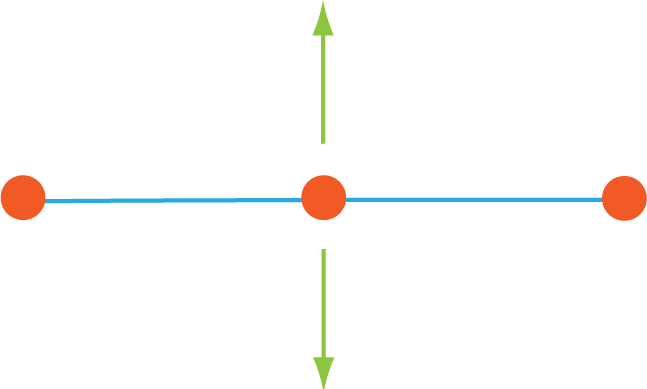
\includegraphics[width=0.32\columnwidth]{images/points1.png}}
  	\subfigure[]{\label{fig:points2}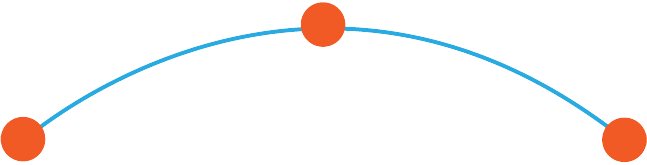
\includegraphics[width=0.32\columnwidth]{images/points2.png}}
  	\subfigure[]{\label{fig:points3}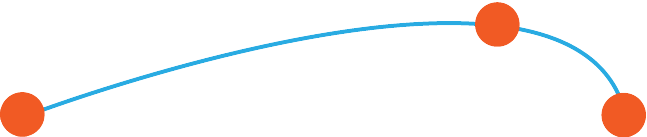
\includegraphics[width=0.32\columnwidth]{images/points3.png}}
  \end{center}
  \caption{Controladores sobre una curva en la imagen. (a) Movimientos posibles de un punto (b) Movimiento del punto central hacia arriba (c) Movimiento no permitido con el fin de no deformar las proporciones de la imagen}
  \label{fig:pointss}
\end{figure}

En la siguiente secci\'on se explican los detalles de implementaci\'on de la deformaci\'on de los implantes como im\'agenes 2D.

%%%%%%%%%%%%%%%%%%%%%%%%%%
\subsection{Implementaci\'on}

\subsubsection{Caja Contenedora Orientada al Objeto}

Con el fin de garantizar que el usuario pueda realizar el movimiento sobre los controladores solamente en la direcci\'on contraria al eje mayor de la caja que contiene el implante, ver Figura \ref{fig:pointss}, se emple\'o un OBB (\textit{Oriented Bounding Box}) como estructura de datos.

Cada OBB se representa bajo la siguiente estructura:

\small
\begin{verbatim}
	struct OBB
	{
		Point2d m_center;					//valor central del implante
		float m_halfDistance[2];	//medias distancias en el eje X e Y
		Vector2d m_upVector;			//eje director \#1
		Vector2d m_atVector;			//eje director \#2
	}
\end{verbatim}
\normalsize

Donde \verb|m_center| representa el valor $(x,y)$ central del implante en dos dimensiones y \verb|m_halfDistance| los valores medios en direcci\'on de los vectores directores del OBB, \verb|m_upVector| y \verb|m_atVector|. Los controladores que ser\'an la gu\'ia para la deformaci\'on se distribuyen a lo largo del eje mayor del OBB.


\subsubsection{Distribuci\'on de los Controladores}

En nuestra propuesta, los controladores son colocados autom\'aticamente, ubicando la mayor cantidad de ellos en una de las siguientes formas:
\begin{enumerate}
	\item En uno de los extremos del implante.
	\item A lo largo de ambos extremos del implante.
	\item A lo largo de la parte central del implante.
	\item Uniformemente a lo largo del eje mayor del implante.
\end{enumerate}

Colocar la mayor\'ia de los controladores sobre un sector espec\'ifico de los implantes permite tener mayor control sobre la deformaci\'on en dicho sector. En este trabajo, nos referimos a la mayor\'ia de los implantes como el $60-70\%$ del n\'umero total de los controladores utilizados. En la Figura \ref{fig:distribution1} se observan diez controladores colocados a lo largo del eje mayor de un implante. Al mover el punto $B$, la deformaci\'on no afecta gran parte de la imagen sino una \'area peque\~na alrededor del controlador. Por otra parte, al mover el controlador $A$ la deformaci\'on afecta el \'area que se encuentra entre sus dos controladores vecinos. Siendo afectada por la deformaci\'on un \'area de mayor tama\~no. 
\begin{figure}[htb]
	\centering
	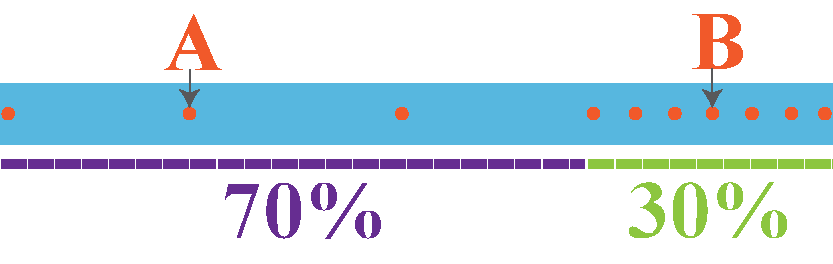
\includegraphics[width=0.60\columnwidth]{images/distribution1.png}
	\caption{Un ejemplo de la distribuci\'on de controladores en un extremo del implante. Siete controladores son colocados uniformemente en un \'area que corresponde al $30\%$ de la longitud del implante. Los otros tres controladores se distribuyen en el restante $70\%$}
	\label{fig:distribution1}
\end{figure}

Para la primera opci\'on de la distribuci\'on de los controladores, la mayor\'ia de los controladores son colocados en los primeros $k$ mil\'imetros en un extremo del implante. El valor de $k$ corresponde al $25-30\%$ de la longitud del eje mayor de dicho implante. Un ejemplo se observa en la Figura \ref{fig:distribution1}, donde se han colocado 7 implantes (de un total de 10) en el \'area correspondiente al $30\%$ de la longitud del implante. El resto de los implantes son distribuidos uniformemente a lo largo del restante $70\%$ de la longitud de eje del implante.

Se aplica un criterio similar para la segunda y tercera opci\'on. Para la segunda opci\'on, ver Figura \ref{fig:distribution2}, la mitad de la mayor\'ia de los controladores son colocados en los primeros $k$ mm. desde un extremo del implante, y la otra mitad en el otro extremo. Para la tercera opci\'on, la mayor\'ia de los controladores son colocados en un \'area de $k$ mm. centrados en la parte media del eje de mayor longitud del implante, como se aprecia en la Figura \ref{fig:distribution3}.
\begin{figure}[htb]
	\centering
	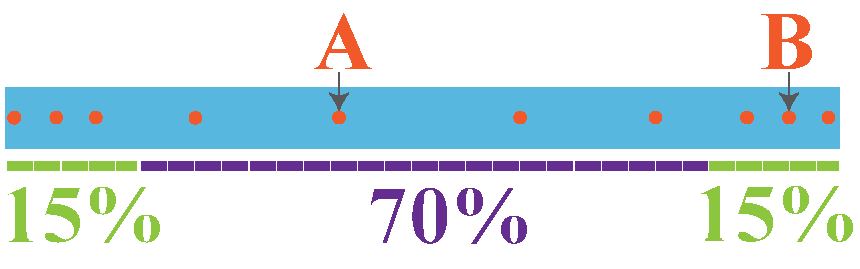
\includegraphics[width=0.60\columnwidth]{images/distribution3.png}
	\caption{Un ejemplo de la distribuci\'on de controladores en cada extremo del implante. Tres controladores son colocados en cada extremo de manera uniforme en un \'area que corresponde al $15\%$ de la longitud del implante. Los restantes cuatro controladores se distribuyen en el restante $70\%$}
	\label{fig:distribution2}
\end{figure}

\begin{figure}[htb]
	\centering
	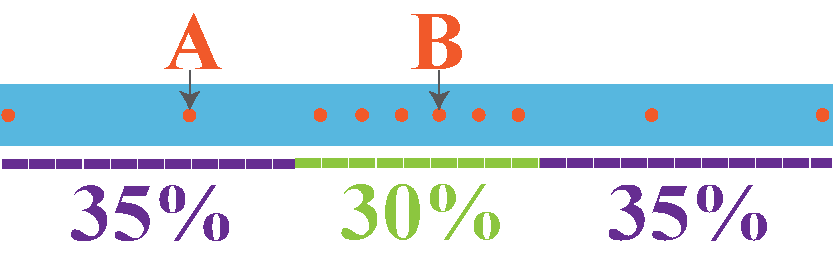
\includegraphics[width=0.60\columnwidth]{images/distribution2.png}
	\caption{Un ejemplo de la distribuci\'on de controladores en centro del implante. Seis controladores son colocados en la parte central dentro de un \'area que corresponde al $30\%$ de la longitud del implante. Los restantes cuatro controladores se distribuyen en ambos extremos, $35\%$ y $35\%$}
	\label{fig:distribution3}
\end{figure}

La \'ultima opci\'on se utiliza en los casos en donde la deformaci\'on debe ser realizada en un lugar distinto a los extremos o la parte media del implante. Estos casos son poco comunes, pero pueden ocurrir. Para ello, los controladores son colocados equidistantemente uno de otro a lo largo del eje mayor del implante.

\subsubsection{\textit{Moving Least Squares}} \label{MLSMalla}

La implementaci\'on de la deformaci\'on con \textit{Moving Least Squares} se realiza empleando cuatro funciones b\'asicas:
\begin{enumerate}
	\item \textit{CrearMLS}: Es ejecutada para crear las estructuras de datos din\'amicas necesarias a ser utilizadas en el MLS.
	\item \textit{Precalcular}: Calcula los valores iniciales del MLS para un estado de reposo inicial (sin deformaci\'on) del implante.
	\item \textit{ActualizarQ}: Cuando el usuario modifica los controladores sobre la curva en el implante para realizar la deformaci\'on, los puntos $q$ expresados en la Ecuaci\'on \ref{ec:principal} son modificados. Esta funci\'on se encarga de actualizar los valores del MLS para estos cambios.
	\item \textit{Dibujar}: Despliega la imagen correspondiente a la deformaci\'on realizada.
\end{enumerate}

A continuaci\'on se explicar\'a cada una de las funciones en m\'as detalle.

\paragraph{\textit{CrearMLS:}} Consiste en crear las estructuras de datos necesarias a ser empleadas durante el algoritmo de deformaci\'on. En esta etapa, se crea una malla uniforme sobre la imagen de acuerdo a un par\'ametro \verb|m_step| que determina el nivel de subdivisi\'on de dicha malla. En la Figura \ref{fig:gridunif}, se muestra un ejemplo de ello.

\begin{figure}[htb]
	\centering
	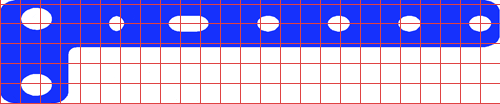
\includegraphics[width=0.70\columnwidth]{images/grid.png}
	\caption{Subdivisi\'on de la imagen del implante en una malla uniforme}
	\label{fig:gridunif}
\end{figure}

La creaci\'on de la malla es con el objetivo de reducir el n\'umero de puntos de la imagen, es decir, tener una menor cantidad de puntos a la que se aplica la deformaci\'on. Este factor reduce considerablemente el n\'umero de c\'alculos a ejecutar por el algoritmo de deformaci\'on. En nuestra propuesta empleamos los controladores como \'unicos puntos de deformaci\'on que afectan a la malla.

Se realiza la deformaci\'on de los puntos que forman la malla, y seguidamente se deforman los p\'ixeles contenidos dentro de cada uno de los cuadros del mallado empleando interpolaci\'on bilineal. La interpolaci\'on bilineal se realiza para los $NxM$ puntos que forman la imagen.

\paragraph{\textit{Precalcular:}}

La deformaci\'on consiste en aplicar la transformaci\'on r\'igida mostrada en la Ecuaci\'on \ref{ec:rigidtransf}. En dicha ecuaci\'on, es posible calcular ciertos valores que ser\'an constantes para la ejecuci\'on de la deformaci\'on si el n\'umero de puntos iniciales no es modificado.
\begin{algorithm}[thp]
	\caption{Precalcula un conjunto de valores a emplear en la deformaci\'on}
	\label{alg:precalcular}
	\begin{algorithmic}[1]
	\Procedure{Precalcular}{$p$}
		\State \textbf{var} Matriz A[4][4]
		\For {cada fila $F$ en la malla $G$}
			\For {cada columna $C$ en la malla $G$}
				\State $w_i \gets \frac{1}{\mid p_i - P_{F,C} \mid^{2 \alpha}}$
				\State $p_{*} \gets \frac{\sum{w_i p_i}}{\sum{w_i}}$
				\State $\hat{p} \gets p_i - p_{*}$
				\State $A[1][1] \gets \hat{p_i} w_i (P_{F,C} - p_i)$
				\State $A[1][2] \gets \hat{p_i} w_i -(P_{F,C} - p_i)^{\perp}$
				\State $A[2][1] \gets \hat{p_i}^{\perp} w_i (P_{F,C} - p_i)$
				\State $A[2][2] \gets \hat{p_i}^{\perp} w_i -(P_{F,C} - p_i)^{\perp}$
			\EndFor
		\EndFor
		\State \textbf{return} $w,p_*,\hat{p},A$;
	\EndProcedure
	\end{algorithmic}
\end{algorithm}

Al precalcular ciertos valores, se disminuye el tiempo de respuesta del algoritmo y hace la deformaci\'on interactiva. En el Algoritmo \ref{alg:precalcular} se muestran las operaciones efectuadas en esta etapa.

En el algoritmo se precalculan los valores de $\hat{p}$ y la matriz $A$. El valor de $p$ est\'a representado en el Algoritmo \ref{alg:precalcular} como $P_{F,C}$, ver Ecuaci\'on \ref{ec:rigidandA}. Se puede observar que el valor de $\hat{p} = \mid P_{F,C} - p_* \mid$ solamente depende de los puntos iniciales $p$ colocados a lo largo del eje mayor del implante. Al mismo tiempo, la matriz $A$ empleada en el c\'alculo de $\vec{f_r(v)}$ depende \'unicamente de $v$ y $P_{F,C}$.

Finalmente, en esta etapa se ejecuta la Ecuaci\'on \ref{ec:rigidtransf} de deformaci\'on r\'igida para el estado inicial, es decir, los puntos $q$ son los mismos puntos $p$ y se obtiene como resultado la imagen original sin deformaci\'on.

\paragraph{\textit{ActualizarQ:}}

Cuando el usuario modifica los controladores en el implante, los valores de $q$ deben ser actualizados. Esto implica recalcular nuevamente los valores de $\hat{q}$ y $q_{*}$. A continuaci\'on se presenta el Algoritmo \ref{alg:actualizarq} con las operaciones aplicadas.

\begin{algorithm}[thp]
	\caption{Actualiza los valores $q_i$}
	\label{alg:actualizarq}
	\begin{algorithmic}[1]
	\Procedure{ActualizarQ}{$w, p_{*},A$}
		\State $min \gets +\infty$
		\State $max \gets -\infty$
		\For {cada fila $F$ en la malla $G$}
			\For {cada columna $C$ en la malla $G$}
				\State $q_{*} \gets \frac{\sum{w_i q_i}}{\sum{w_i}}$
			\State $\hat{q} \gets q_i - q_{*}$
			\State $\vec{f_r(P_{F,C})} \gets \sum_i{ \hat{q_i} A_i}$
			\State $f_r(P_{F,C}) \gets \mid P_{F,C} \mid - p_{*} \frac{\vec{f_r(P_{F,C})}}{\mid \vec{f_r(P_{F,C})} \mid} $
			\If{$f_r(P_{F,C}) < min$}
					$min \gets  f_r(P_{F,C})$
			\EndIf
			\If{$f_r(P_{F,C}) > max$}
					$max \gets  f_r(P_{F,C}) $
			\EndIf
			\EndFor
		\EndFor
		\State \textbf{return} $min, max$;
	\EndProcedure
	\end{algorithmic}
\end{algorithm}

En el Algoritmo \ref{alg:actualizarq}, se modifican los puntos $P_{F,C}$ de la malla $G$ a una nueva ubicaci\'on $P^{'}_{F,C}$ (los cuales son sobreescritos). Esto origina nuevas posiciones $x,y$ dentro de la imagen empleando los valores $w,p,A$ y calculando $q_*$ y $\hat{q}$ para las posiciones actuales de los controladores. Adem\'as, el resultado del procedimiento \textit{ActualizarQ} retorna 2 valores de la nueva imagen: $min = (x_{min},y_{min})$ y $max = (x_{max},y_{max})$.

Con estos valores, es posible formar una imagen de dimensiones $(W,H) = (x_{max} - x_{min}, y_{max} - y_{min})$ la cual es creada din\'amicamente cuando las dimensiones sean distintas a las dimensiones de la imagen original. Una vez creada la nueva imagen, se realiza una correspondencia entre cada punto de la malla de la imagen nueva $P^{'}_{F,C}$, con los puntos de la malla de la imagen original $P_{F,C}$. El \'ultimo paso es desplegar la imagen para mostrar los resultados.

\paragraph{\textit{Dibujar:}}

Una vez que se han obtenido los nuevos puntos de la deformaci\'on de la malla, como se observa en la Figura \ref{fig:grid}, se procede a realizar la correspondencia entre cada uno de los p\'ixeles internos de dicho implante.
\begin{figure}[htbp]
  \begin{center} 
  	\subfigure[]{\label{fig:grid1}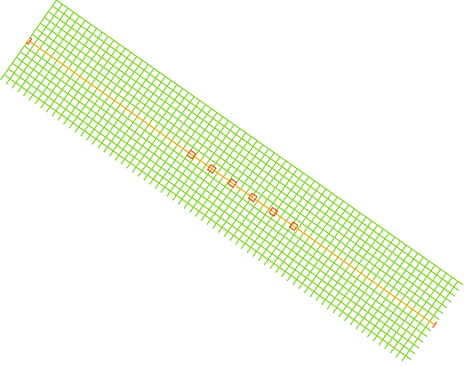
\includegraphics[width=0.30\columnwidth]{images/grid1.png}}
  	\subfigure[]{\label{fig:grid2}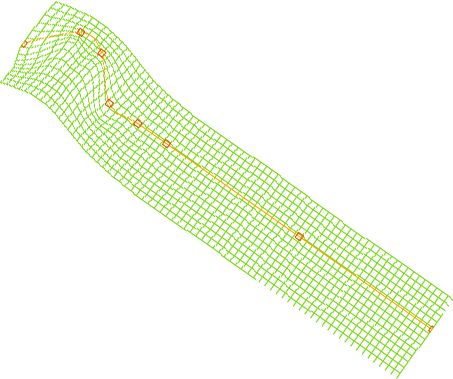
\includegraphics[width=0.30\columnwidth]{images/grid2.png}}
  \end{center}
  \caption{Malla correspondiente a un implante en (a) su estado original, y (b) con la deformaci\'on aplicada}
  \label{fig:grid}
\end{figure}

Si la imagen es subdividida en $M \times N$ puntos en la malla, entonces se tendr\'an $M - 1 \times N - 1$ cuadril\'ateros. A su vez, cada cuadril\'atero se subdivide en dos tri\'angulos como se observa en la Figura \ref{fig:baryc}.

\begin{figure}[htbp]
	\centering
	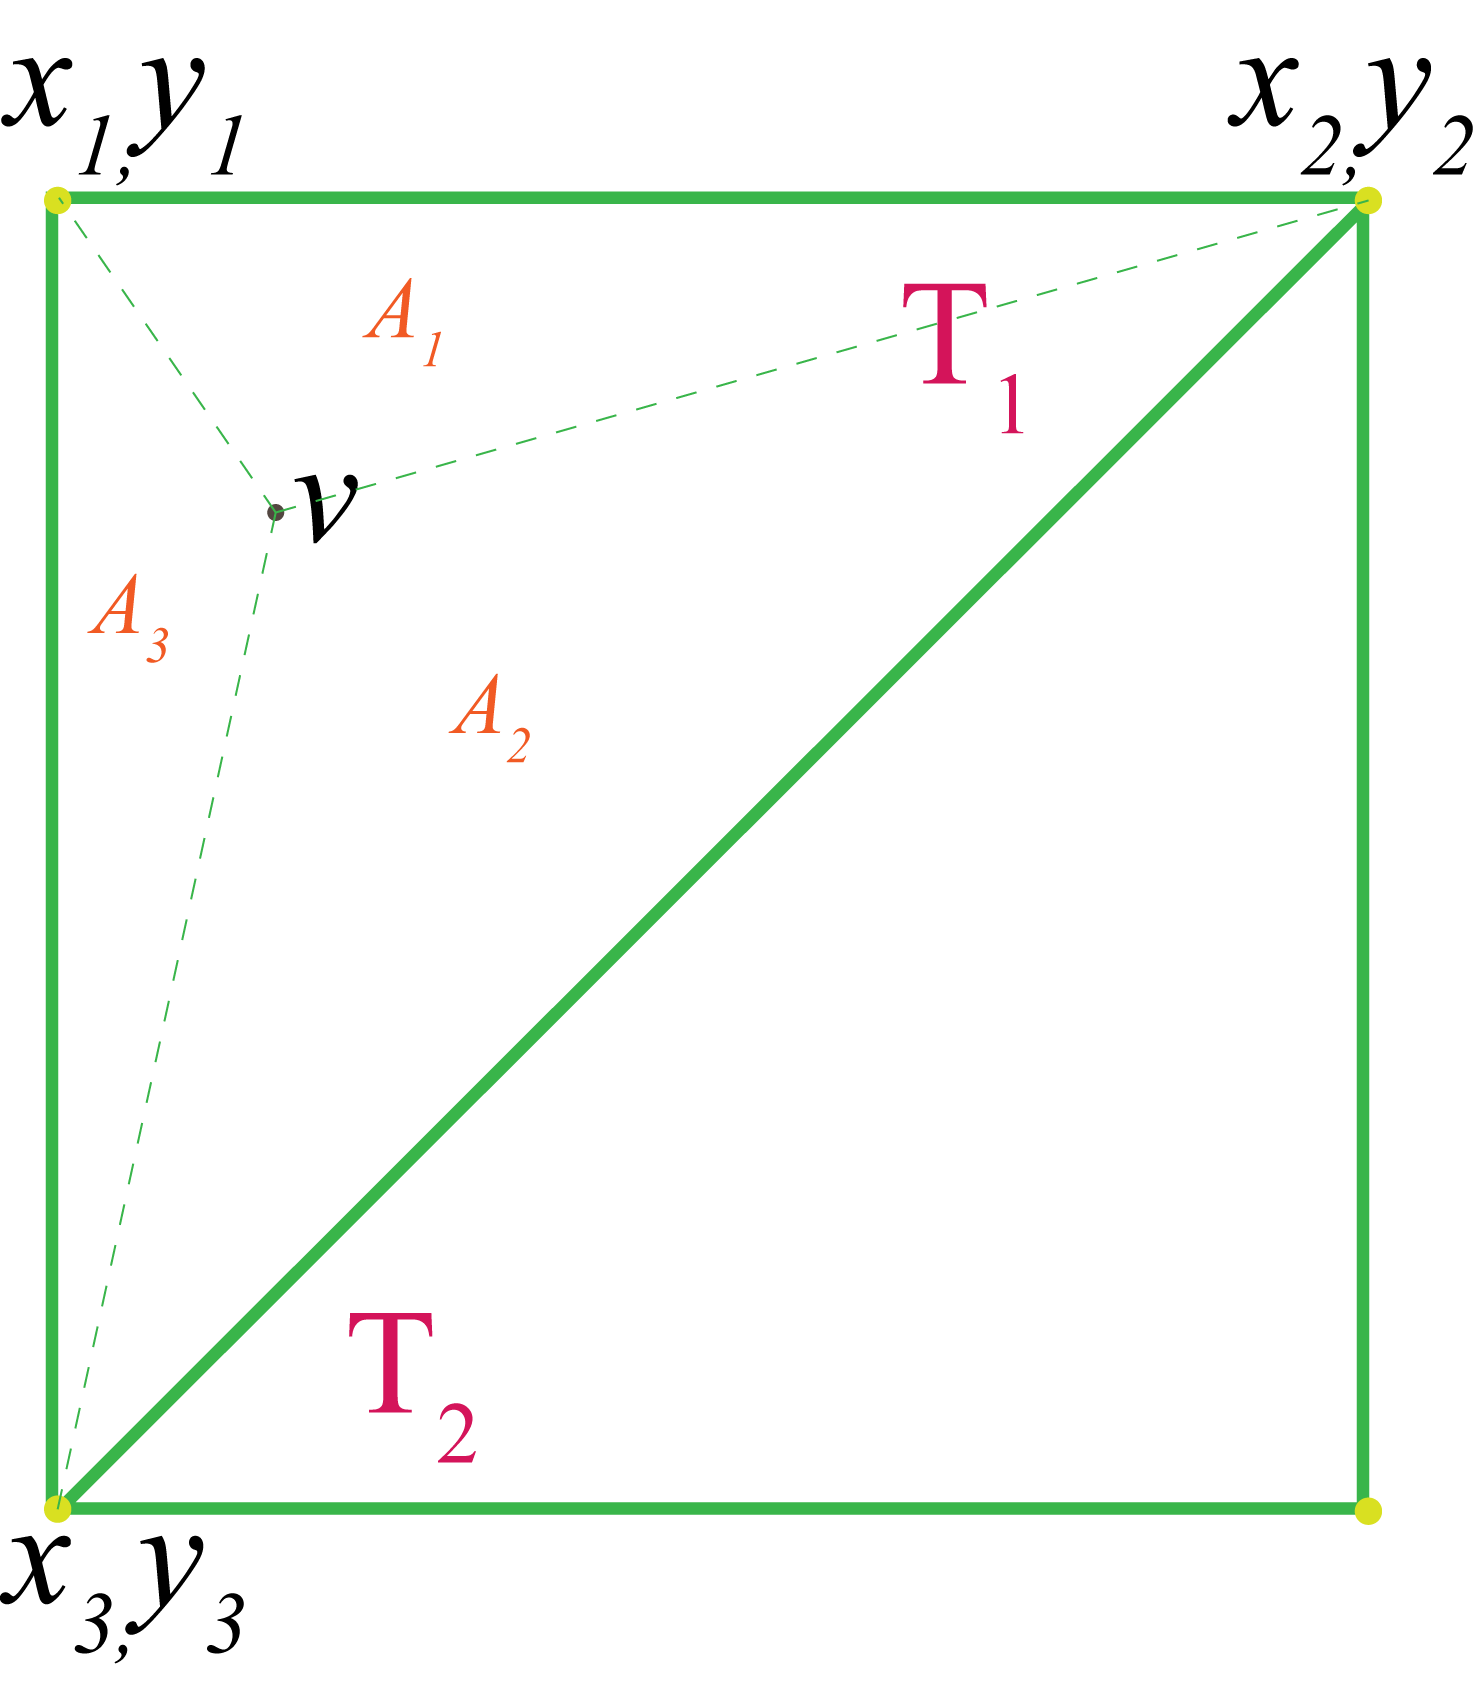
\includegraphics[width=0.35\columnwidth]{images/barycentric.png}
	\caption{Cuatril\'atero subdividido en dos tri\'angulos y ubicaci\'on de un punto $v$ sobre uno de ellos}
	\label{fig:baryc}
\end{figure}

Para dibujar los p\'ixeles internos de la nueva malla, se emplean coordenadas baric\'entricas para ubicar el aporte de un p\'ixel $v$ con respecto al tri\'angulo donde yace en la imagen original, sobre la imagen deformada. Para ubicar las coordenadas baric\'entricas de un punto $v$ sobre un tri\'angulo, se realiza la interpolaci\'on de los tres puntos que forman el mismo, ver Figura \ref{fig:baryc}.

Un punto $v$ se define como $v = \sum_{i=1}^{3}{\varphi_{i}(v)v_i}$, donde $\varphi_i(v)=\frac{A_i(v)}{A_1(v) + A_2(v) + A_3(v)}$. Para el caso de un tri\'angulo, se tienen 3 puntos definidos como $v_1=(x_1,y_1)$, $v_2=(x_2,y_2)$ y $v_3=(x_3,y_3)$. Para verificar que un punto $v$ se encuentre dentro del tri\'angulo formado por $\triangle v_1 v_2 v_3$, se debe cumplir que $\varphi_{i} > 0$ y $\sum_{i=0}^{3}{\varphi_{i}} = 1$.

Una vez realizado este proceso se obtiene el resultado final que consiste en la imagen deformada en base a los controladores modificados por el usuario. El proceso de deformaci\'on del implante, debe ser lo m\'as parecido a como se realiza en una sala de operaciones. La forma de comprobar la similitud de dicho proceso es a trav\'es de los m\'edicos cirujanos. En el siguiente cap\'itulo, se presenta una serie de pruebas tanto para la deformaci\'on de los implantes dentro de nuestra propuesta como de otros algoritmos. Al mismo tiempo, se presentar\'an los resultados obtenidos de dichos experimentos.